\section{Empirical Results}
\label{sec:bleuresult}

In this section, we present the empirical results to validate our hypothesis that
\textit{BLEU is not effective in evaluating translation quality of source code migration task}.
\subsection{Correlation between BLEU and Semantic scores}
To justify the first part of our hypothesis, BLEU score does not reflect well
the semantic accuracy of results translated by a particular model,
we show the relation between BLEU scores and human judgments via semantic scores.
We use Pearson's correlation coefficient~\cite{PearsonCorrelation} to gauge
how strong their relation is. The correlation coefficient has value
between [-1, 1], where 1 indicates the strongest positive relation, -1
indicates the strongest negative relation, and 0 indicates no relation.

Fig.~\ref{fig:BleuSemlpSMT} and Fig.~\ref{fig:BleuSemMppSMT} show the
scatter plots between two metrics: BLEU and Semantic. Each point
represents the scores of a pair of methods where its $x$-axis value is
for BLEU scores and $y$-axis value is for semantic scores. The
correlation coefficient between BLEU and semantic scores for the model
mppSMT is 0.523 and for the model lpSMT is 0.570. These positive values
are closer to 0.5 than to 1.0. This means there is a {\bf positive but weak
relation} between BLEU score and semantic score. The weak correlations %help me to check grammar
between the metrics on the results translated by lpSMT and mppSMT are
demonstrated in Fig.~\ref{fig:BleuSemlpSMT} and Fig.~\ref{fig:BleuSemMppSMT}.

%\emph{Observation 1:}

\subsubsection{{\bf Higher BLEU does not necessarily lead to higher
sematic accuracy}}

In Fig.~\ref{fig:BleuSemlpSMT}, it is clear that for many specific
values of BLEU, the corresponding semantic scores can spread out in a
wide range. For instance, the BLEU score of 0.75, the corresponding
semantic scores are from 0.25 to 1.
% \textbf{Ngoc: can u mark in the figure please}.
Thus, from this observation, we conclude that the results migrated by
these models with {\em high BLEU scores might not achieve high semantic
scores}.
%There are two reasons for this.
%

%In our sample set, these results can fall in two main cases.
There are two main reasons for this result in our dataset.  First, the
translated methods might have multiple correct phrases, but in an
incorrect order, those method can be incorrect, even not compilable.
%useless and justified as so in human judgment.
%
For example, in Fig.~\ref{fig:issueexample2}, the translated method
misplaces the position of the bracelet, making the method have low
semantic score, however, it has high BLEU score.
%
%Another reason for this implication is that resulting method does not capture the important
%program elements.
In other cases, the migrated results are incomplete code missing the
elements that are trivial for the translation model, yet important
with respect to the syntactic rules of the target language. For
example, the result contains mostly keywords and separators such as
\code{if}, \code{public}, \code{()}, but misses out the important
program elements such as function calls or variable names. In this
case, it will have low semantic score while having a moderate to high
BLEU score. These circumstances indicate the weakness of BLEU metric
in evaluating the translated results in programming language where
syntax rules are well-defined.

%\emph{Observation 2:} For a fixed value of Semantic score, there can
%be many associated BLEU values. Specifically, in the model lpSMT, with
%a Semantic Score of 1, the BLEU scores can vary greatly between 0-1,
%which is reflected on the top horizontal line of dots in the
%Figure~\ref{fig:BleuSemlpSMT}. Similarly, in
%Figure~\ref{fig:BleuSemMppSMT}, with the Semantic Score of 1, the BLEU
%scores are in the range of 0.5 to 1.

\subsubsection{{\bf Higher semantic accuracy does not necessarily lead to
higher BLEU score}} In the results translated by mppSMT
(Fig.~\ref{fig:BleuSemMppSMT}), for a particular value of semantic
score, there can be many corresponding BLEU values spreading out in
a~wide range. Specifically, with the semantic score of 1, the BLEU
scores can vary from 0.5 to 1.0. Thus, it can be concluded
that for this model, the migrated code achieving {\bf higher semantic score does not necessarily has higher BLEU~score}.

%From this observation, it can be implied that translated code can have
%low BLEU score, but high Semantic score. This can be explained by two
%reasons.
From our data, we observe that there are two main reasons leading to
that result.
%
First, a translated method can use code structure different from the
reference one to perform the same
functionality. Fig.~\ref{fig:mppSMT_example} shows an example that got
a maximum semantic score, but has low BLEU score of 0.4. In this
example, the translated method uses a \code{for} loop instead of a
\code{foreach} loop as in the reference code. The second reason
for this phenomenon is the whitespace issue. For example, in
Fig.~\ref{fig:mppSMT_example}, the translated code has the tokens
\code{IsSimilar(}, but the reference code has \code{IsSimilar (}. The
former is interpreted as one token while the latter is interpreted as
two tokens.  This situation reduces the precision on phrases, but the
human subject still evaluated the result with high semantic score. By
this experiment, we also empirically verify that the focus on the
lexical precision of BLEU makes it unable to capture other
code-related aspects such as program dependencies that contribute to
source code semantics. This might lead to the ineffectiveness of BLEU
in reflecting the semantic accuracy of translated results.

%TODO need to verify
In conclusion, {\em BLEU does not reflect well the
semantics of source code, and it is not suitable in evaluating
semantic accuracy of the result from a SMT-based code migration model}.

\begin{figure}[t]
\centering
%\begin{lstlisting}[basicstyle=\small\sffamily, stepnumber=1, numbers=left, language=Java, aboveskip=1pt,  belowskip=1pt, numbersep=-5pt]
\lstinputlisting[basicstyle=\scriptsize\sffamily,language=Java]{mppExample.cs}
%\end{lstlisting}
\caption{mppSMT Example}
\label{fig:mppSMT_example}
\end{figure}


\subsection{The use of BLEU in comparing SMT migration models}

%TODO complete and describe t-test results
To confirm the difference in the semantic scores for the two
models even though they have the same BLEU~score, we performed the
paired $t$-test\cite{geek_2015} on those 375 results with the confident level of
0.95 and a null hypothesis that {\em the semantic scores of two models
are equal}. With such setting, the t-critical value is 1.967, and for this data set, the confident interval for the difference between the mean semantic scores of two models is $\pm0.04$. It means the difference must be larger than 0.04 to be considered significant. The $p$-value (the probability 
that the results occurred by chance) of our test is 2.81E-85, which is much
smaller than significant level of 0.05. Thus, we rejected the null hypothesis and concluded
that the semantic scores of two models are different with the confident
level of~95\%.

%TODO gonna be removed
Additionally, in our experiment on results translated by mppSMT and 
p-mppSMT, the average BLEU score for these models are
identical. Meanwhile, the overall semantic score for p-mppSMT is
\textbf{0.62}, which is lower than the average for mppSMT of
\textbf{0.88}. This means that the deviant of BLEU in comparing the
two models is nearly \textbf{2} levels of semantic score lower,
despite that they have identical BLEU score.

%To evaluate the abilities of BLEU in comparing the 
%translation quality of models, we show that the two models mppSMT and p-mppSMT have different semantic score despite having identical BLEU score. We perform the paired t-test on the sample with confident level of 0.95. Our null hypothesis is the semantic scores of two models are equal. The p-value of the t-test is 2.81E-85
%which is much smaller than 0.05. Thus we reject our null hypothesis and conclude that the semantic scores of two models are different with confident level of 95\%.


%Tien
%In our dataset, there are two main reasons for these results. First,
%in some results of mppSMT, these phrases are lexically different those
%in the reference one, but they may carry correct syntactical or
%semantic information, which makes these results achieve high semantic
%score. However, for the results translated by p-mppSMT and having
%similar BLEU scores, these meaningful phrases are swapped, thus, are
%placed in incorrect locations. This leads to significantly decreasing
%in semantic scores. For example, in Fig.~\ref{fig:mppSMT_example}, the
%result translated by p-mppSMT which has the same BLEU score with the
%result of mppSMT. Meanwhile, the result of mppSMT is semantically
%correct, however, the result from p-mppSMT is not compilable.
%
%Furthermore, although several result of mppSMT might contain phrases
%that are lexically incorrect, these phrases have the information that
%provides developers clues to fix the translated one. However, these
%phrases in the corresponding results translated by p-mppSMT are moved
%into new positions, which also makes the semantic score of these
%results are much lower than that of mppSMT. For example,...
%\textbf{NGOC, example for this reason}

Examining the translated code, we found that p-mppSMT produces the
code with lower semantic accuracy due to the swapping of the locations
of the expressions and/or statements in the code. That leads to the
completely different program semantics and even incompilable code. For
example, in Fig.~\ref{fig:mppSMT_example}, the phrase with the method
name \code{isSimilar} is placed in the end of line 28, making the code
incorrect. Therefore, the semantic score of such result is lower
than the result from mppSMT.

%




%\subsubsection{Theoretical Models}
%To prove the second part of our hypothesis, we conduct study to see if an improvement in BLEU score over models reflects the improvement in translation quality represented by human judgments of semantic score. For a same set of 375 original Java methods, the two models mppSMT and mppSMT2 generates two sets of 375 translated methods. Each set has its own BLEU scores and Semantic scores. 
%From the 375 pairs, we have 73 pairs that have identical BLEU scores but are different in term of lexical. 26 out of 73 (\textbf{35\%}) have lower semantic score. On average, semantic score of model mppSMT2 is lower than mppSMT's by 0.16. Given that our semantic scores have only 5 pivots range from 0 to 1, a deduction of 0.16 is a large margin as it nearly reduces the semantic score by one pivot point.  
%The model mppSMT2 would swap the positions of incorrect phrases in term of lexical. However, those phrases may still have semantic information as the model mppSMT is capable of produce code that are semantically correct but lexically incorrect. There are many cases that they are semantically incorrect but still help the whole translated code syntactically correct or provide users with good starting point for the migration task. We have showed that a theoretical model can achieve identical BLEU score but has lower translation quality compared to another. 
%\subsubsection{Practical Models}

%Using the same experiment set up, we have two sets of 375 translated methods from two models GNMT and mppSMT. From the sample, we choose pairs of results such that their GNMT's BLEU scores are higher than mppSMT's BLEU scores. There are 215 of such pairs. Among them, 79 pairs have lower semantic score. Then, we perform t-test with alpha confident level of 0.95 on that subset to see if their GNMT's semantic scores are also significantly higher or not. Our null hypothesis is: GNMT's semantic score are higher than mppSMT's one with confident level of 0.95. The results show a t-value of \textbf{-9.1} which is lower than the critical point of -1.97. It meant we would reject the null hypothesis that GNMT's semantic scores are higher than mppSMT's ones. Our result shows that an improvement in BLEU score does not lead to an improvement in translation quality. 

%To validate the use of BLEU in comparing different SMT-based code migration systems, we conduct study to see if an improvement in BLEU score over cross models reflects the improvement in translation quality represented by human judgments of semantic score between those models. For a same set of 375 original Java methods, the two models GNMT and mppSMT generates two sets of 375 translated methods. Each set has its own BLEU scores and Semantic scores.
%We prove that an improvement in BLEU score does not sufficient nor necessary lead to an improvement in semantic score by showing:
%
%1. From the sample, we choose pairs of results such that their GNMT's BLEU scores are higher than mppSMT's BLEU scores. Then, we perform t-test with alpha confident level of 0.95 on that subset to see if their GNMT's semantic scores are also higher or not. The results show a t-value of ... It meant we would reject the null hypothesis that GNMT's semantic scores are higher than mppSMT's ones. So, it can be concluded that an improvement in BLEU score is not sufficient to achieve a higher semantic score. 
%
%2.  From the sample, we choose pairs of results such that their mppSMT's semantic scores are higher than GNMT's semantic scores. Then, we perform t-test with alpha confident level of 0.95 on that subset to see if their mppSMT's BLEU scores are also higher or not. The results show a t-value of ... It meant we would reject the null hypothesis that mppSMT's BLEU scores are higher than GNMT's ones. So, it can be concluded that an improvement in BLEU score is not necessary to achieve a higher semantic score. 

%We ignored pairs of translated results if they have the same BLEU score or Semantic score (136 of the cases). For the remaining results, we found out that in \textbf{34\%} of the cases, the change in BLEU score contradicts the change in Semantic score. It means an improvement in BLEU score leads to a decrease in Semantic score and vice versa. In other words, if one function is translated by two migration models, one-third of the time, the result which has higher BLEU score actually has lower translation quality than the other.

%Because of the results above, BLEU is not reliable to use in comparing different SMT-based migration models.

In our work, we additionally conducted another experiment in the same
manner to verify our hypothesis on two pairs of SMT-based migration
models: lpSMT~\cite{fse13} and GNMT~\cite{gnmt}, and
mppSMT~\cite{ase15} and GNMT~\cite{gnmt}. The results from our
$t$-tests allowed us to conclude that an improvement in BLEU score is
not sufficient nor necessary to reflect a higher semantic score with
the confidence of 0.95. Thus, the experimental results also support
our hypothesis. The details of this study can be found on our
website~\cite{ruby-website}.

In brief, we conclude that \textit{BLEU is not effective in comparing
  the translation quality of SMT-based models}.


\begin{figure}
\caption{BLEU metric vs Semantic metric (lpSMT model)}
\centering
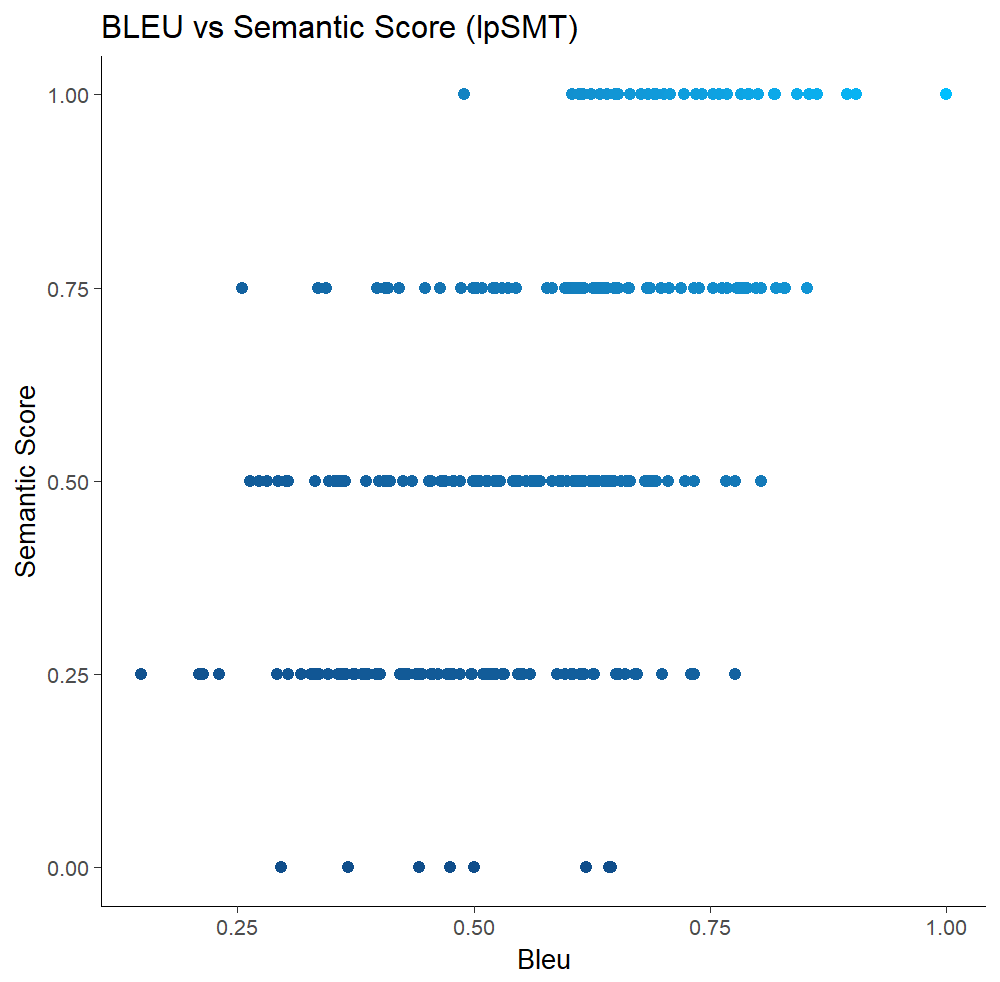
\includegraphics[scale=0.5]{img/bleuvssemantic_lpSMT.png}
\label{fig:BleuSemlpSMT}
\end{figure}

\begin{figure}
\caption{BLEU metric vs Semantic metric (mppSMT model)}
\centering
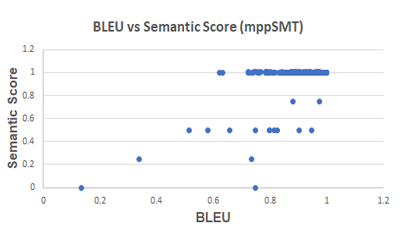
\includegraphics[scale=0.5]{img/bleuvssemantic_mppSMT.png}
\label{fig:BleuSemMppSMT}
\end{figure}

